\section{Architecture for Embedded Software Verification}\label{architecture_s}	
Figure~\ref{architecture} presents the overall proposed architecture for ensuring Java bytecode correctness. 
\begin{figure}[ht!]
\begin{center}
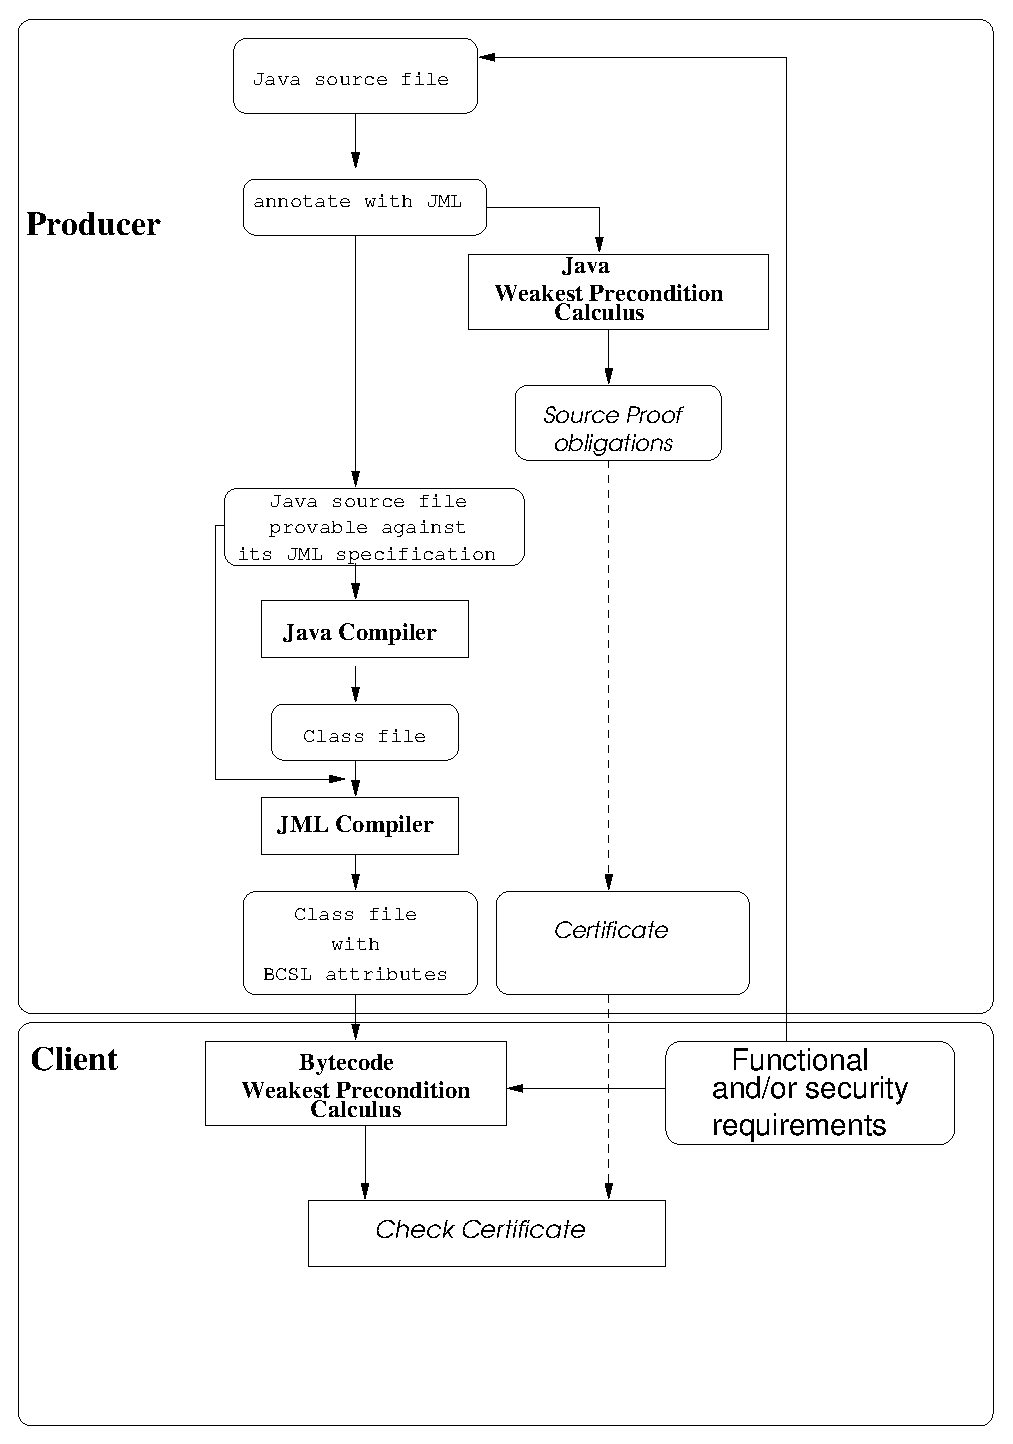
\epsfig{file=architecture.eps, width=\linewidth}
\caption{The overall architecture of the annotating and verifying code}
\label{architecture}
\end{center}
\end{figure}
The process starts with a Java source file annotated by the code producer with JML assertions. 
This code and the annotations are checked with respect to an API given by the client through a verification tool running at source level such as JACK.
The API can consist on some restricted services used by the application or on an annotated interface that the application must implement. 
When the annotation are sufficient to prove the code, the Java file is then normally compiled with a Java compiler to obtain a class file. 
This class file is then annotated with special JML attributes extracted from the source file. 
The code can then reach the client side where proof obligations are generated (at code level) with respect to client's API requirements. 
The corresponding proof obligations are then proved, for instance, with the JACK framework. If the client succeeds in proving the verification conditions, he can trust the unknown code. 
%As is shown on the figure~\ref{architecture} in the general case we do not specify who does the proof. It may be the client, the code producer or a third party. Here in this paper we consider that it is the client that genrates the proof.
In this framework, it is not necessary for the client to have an access to the source to verify high level properties. 
Nevertheless those properties can be expressed easily at source level.

To implement this framework, we have defined an extension of the class file format and we have implemented a tool to insert those special attributes in the class file. The next section introduces those extensions.  

